\chapter{What It Is}

To assist us in the experimental analysis of different algorithms and method, we developed a simulator called \RSS. The main aspects considered during its development are:
\begin{quote}
	\begin{itemize}
		\item Simple Usage
		\item Portability
		\item Simple adding of new robot algorithms
		\item Diversity of useful Features
	\end{itemize}
\end{quote}
In the following we will discuss why and how these aspects emphasize the \RSS as a helpful tool in of research of swarm algorithms (Section~\ref{WII:sec:special}). Afterwards we will name some possible fields of application of the \RSS (Section~\ref{WII:sec:application}).

\section{What makes the \RSS special?}\label{WII:sec:special}

\subsection{Simple Usage}\label{WII:sec:simpleusage}
In theoretical research simulators often are a helpful tool for checking conjectures or assumptions that emerge during research. Since they are an auxiliary tool in the progress of showing and proving new results, one does not want to bother with its usability. Therefore, the \RSS is developed with usability in mind and therefore provides the user with a steep learning curve.\medskip

The \RSS comes with an instance generator, which generates a simulation specification in form of three files: a main project file, a robot file and an obstacle file.
The main project file contains all necessary information about the simulation process. The robot and obstacle file contain information (like position or type) about the robots or obstacles, respectively. See Appendix~B of the \RSS's User's Guide \cite{WII:cite:usersguide} for a detailed description of these files. 
For example, if you want to generate an instance for a simulation with the following properties
\begin{quote}
\begin{itemize}
	\item 1000 robots randomly distributed in a cube of size 20
	\item add a position request handler (which loads a default module for handling the robots' movements)
	\item use \textsc{COGRobot}\footnote{In this algorithm the target position of a robot is the center of gravity of all robots.} as robot algorithm for all robots
\end{itemize}
\end{quote}
the following command generates the according input files for the \RSS:
\lstset{language=C++}
\begin{lstlisting}[numbers=none]
./RobotSwarmSimulator --generate --distr-pos 20 --add-pos-handler --robots 1001 --algorithm COGRobot
\end{lstlisting}
Of course you can also easily edit or generate the files for the input specification by hand.\medskip

Once you have created the input files necessary for the simulation you can run the \RSS using these input files with the following command:
\lstset{language=C++}
\begin{lstlisting}[numbers=none]
./RobotSwarmSimulator --project-file main-project-file-name
\end{lstlisting}
The \RSS (including its instance generator) provides a variety of input parameters, described in Section~2.2 of the \RSS's User's Guide.\medskip

After we have generated input files and started the \RSS with two easy to use commands, a graphical user interface visualizing the robot positions by colored dots appears (Figure~\ref{WII:fig:simulator}).\medskip

\begin{figure}[htp]
\centering
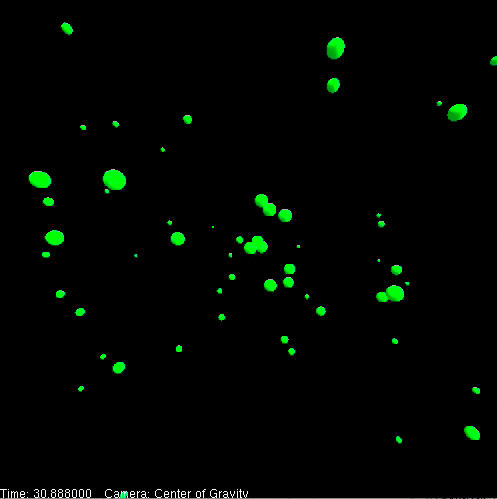
\includegraphics[width=0.5\textwidth]{chapter_whatitis_fig/simulator.png}
\caption{Screenshot of the \RSS running a simulation}
\label{WII:fig:simulator}
\end{figure}
For better observing the robots' movements the User Interface provides different camera modes: 
\begin{quote}
\begin{itemize}
	\item the \texttt{CogCamera}, where the camera is located at the center of gravity of all robots
	\item the \texttt{FollowSwarmCamera}, where the camera moves such that the swarm is always visible
	\item the \texttt{MoveableCamera}, where the user can move the camera's position by mouse or keyboard interactions
\end{itemize}
\end{quote}
More features of the User Interface will be described in Section~\ref{WII:sec:features}.\medskip

\subsection{Portability}
Besides its simple usage the \RSS stands out in its portability: it comes as executable for Windows, Linux and Mac OS X.
We also payed attention that the external libraries we used are also portable to all of these systems. Thus, the development of the \RSS is possible on Windows, Linux and Mac OS X. In addition to theses three systems, it is also easy to port the \RSS to  other UNIX-like operating systems.


\subsection{Simple Adding of New Robot Algorithms}
The \RSS comes with a set of already implemented robot algorithms. Just to name a few, there are 
\textsc{LocalFlow} (Figure~\ref{WII:fig:local-flow}),
\textsc{GridPullSpin} (Figure~\ref{WII:fig:gridpullspin2d}),
\textsc{MovingChain} (Figure~\ref{WII:fig:moving-chain}) or
\textsc{Lattice2DRobot} (Figure~\ref{WII:fig:cloning-movement}).\\

\begin{figure}[ht]
	\centering
	\begin{minipage}[t]{0.46\textwidth}
		\centering
		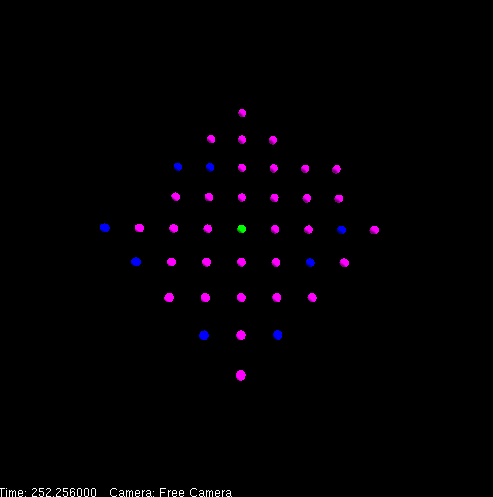
\includegraphics[width=\textwidth]{chapter_whatitis_fig/local-flow}
		\caption{Visualization of the \textsc{LocalFlow} algorithm}
		\label{WII:fig:local-flow}
	\end{minipage}$\quad$
	\begin{minipage}[t]{0.46\textwidth}
		\centering
		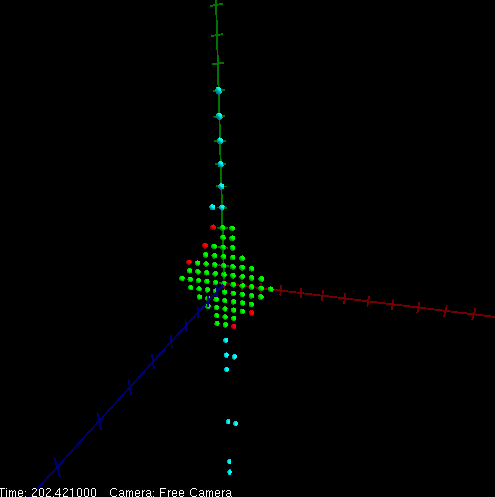
\includegraphics[width=\textwidth]{chapter_whatitis_fig/gridpullspin2d.png}
		\caption{Visualization of the \textsc{GridPullSpin} algorithm with global coordinate system displayed}
		\label{WII:fig:gridpullspin2d}
	\end{minipage}
	\begin{minipage}[t]{0.46\textwidth}
		\centering
		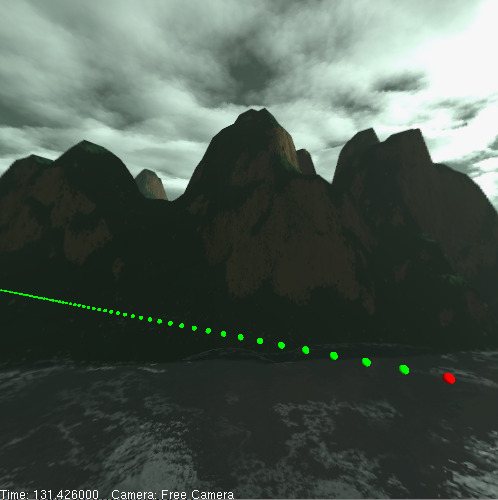
\includegraphics[width=\textwidth]{chapter_whatitis_fig/moving-chain.png}
		\caption{Visualization of the \textsc{MovingChain} algorithm with a textured skybox}
		\label{WII:fig:moving-chain}
	\end{minipage}$\quad$
	\begin{minipage}[t]{0.46\textwidth}
		\centering
		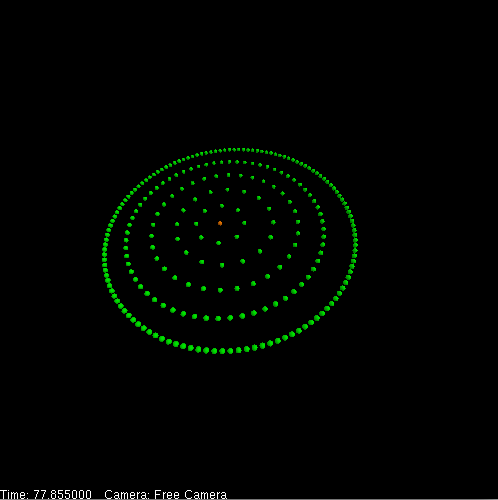
\includegraphics[width=\textwidth]{chapter_whatitis_fig/cloning-movement.png}
		\caption{Visualization of the \textsc{CloningMovement} algorithm}
		\label{WII:fig:cloning-movement}
	\end{minipage}
\end{figure}

But the \RSS is not limited to the predefined robot algorithms. It is easy to add own, new robot algorithms. This can be done by implementing the robot algorithm you want to test in \Cpp or in \Lua. 
In both cases you do not have to work through the whole code or know how the simulator works inside. Thus, you can easily add your new algorithm in just a few minutes to the \RSS.
Section~2.4 of the \RSS's User's Guide provides more information about how to add your own algorithm to the \RSS.

\subsection{Diversity of Useful Features}\label{WII:sec:features}
Besides its simple usage, the computation of statistical measures is a powerful feature of the \RSS. 
If the computation of statistical measures is enabled by the command that runs the \RSS, the statistics defined in the main project file will be generated during the simulation.
There are several supported statistics like average position of the robots, minball center of the robots, minball radius of the robots or maximal distance from the origin, just to name a few. It is also easy to extend the statistics module of the \RSS to support even more statistical measures.
Furthermore, the statistics module of the \RSS is highly adaptable. For instance, one can define, which values will be outputted during a simulation.
\par
For a clear interpreting of the statistical measures or directly inserting the result into a paper, the \RSS provides an automatic generation of GnuPlot charts of the computed measures.\medskip

As already mentioned above, the User Interface of the \RSS provides some further controlling and visualization features. 
The controlling features include the possibility to let the user pause (and resume) the simulation at any time or increase (or decrease) the simulation speed. If an according camera mode is selected (which can as well be done by the user during the simulation) the user is also able to navigate through the scene by mouse or keyboard. \par
The visualization features include some useful presentation possibilities for getting more information. Just to name a few, some of these features are
\begin{itemize}
	\item display the center of gravity of the swarm (Figure~\ref{WII:fig:cog})
	\item display a help screen providing available shortcuts (Figure~\ref{WII:fig:help-screen})
	\item display global or local coordinate systems (Figure~\ref{WII:fig:gridpullspin2d}, Figure~\ref{WII:fig:local-coordinates})
	\item display visibility graph (Figure~\ref{WII:fig:visibility-graph})
	\item single step mode
	\item save current simulation
\end{itemize}
All these features can easily be enabled by shortcuts, which can be displayed in a help screen by simply pressing \texttt{h}.


\begin{figure}[ht]
	\centering
	\begin{minipage}[t]{0.46\textwidth}
		\centering
		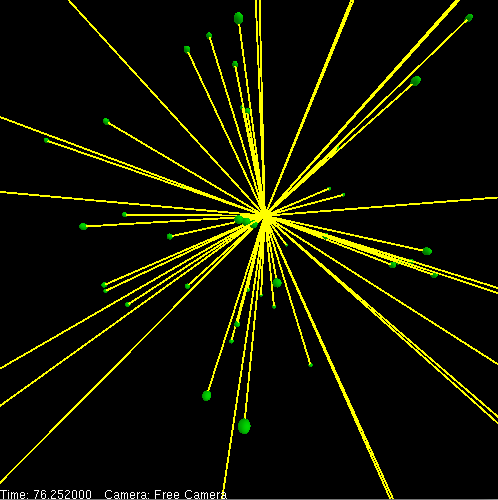
\includegraphics[width=\textwidth]{chapter_whatitis_fig/cog.png}
		\caption{Center of gravity of the swarm}
		\label{WII:fig:cog}
	\end{minipage}$\quad$
	\begin{minipage}[t]{0.46\textwidth}
		\centering
		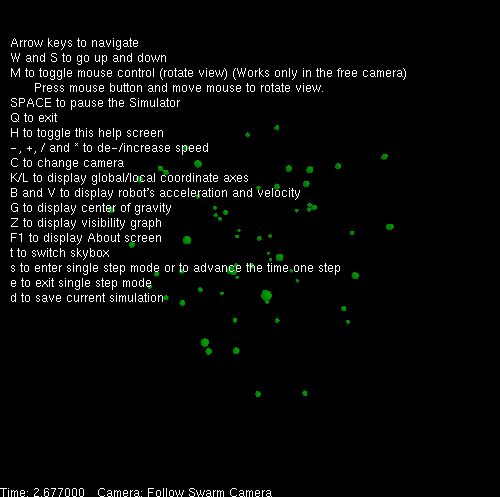
\includegraphics[width=\textwidth]{chapter_whatitis_fig/help-screen.png}
		\caption{Help screen of the \RSS}
		\label{WII:fig:help-screen}
	\end{minipage}
	\begin{minipage}[t]{0.46\textwidth}
		\centering
		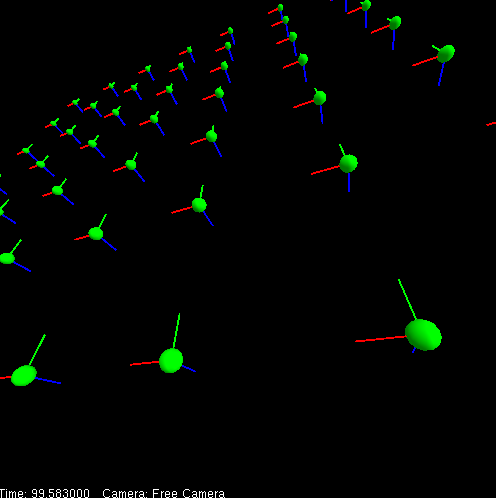
\includegraphics[width=\textwidth]{chapter_whatitis_fig/local-coordinates.png}
		\caption{Local coordinate systems}
		\label{WII:fig:local-coordinates}
	\end{minipage}$\quad$
	\begin{minipage}[t]{0.46\textwidth}
		\centering
		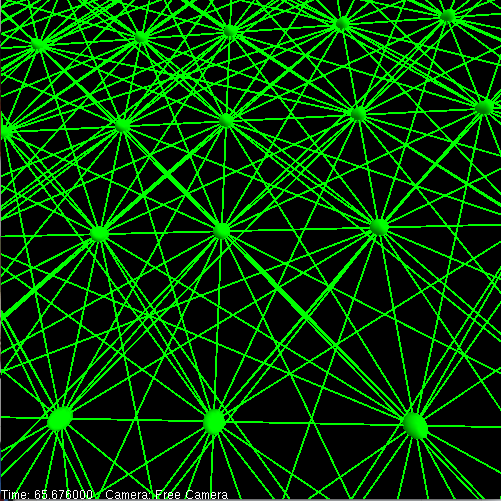
\includegraphics[width=\textwidth]{chapter_whatitis_fig/visibility-graph.png}
		\caption{Visibility graph of robots arranged in a lattice}
		\label{WII:fig:visibility-graph}
	\end{minipage}
\end{figure}


\section{Application Possibilities}\label{WII:sec:application}
In this section we will give some ideas in which areas the \RSS can be a very helpful tool.\par
Imagine, you developed an robot algorithm and want to get an idea of the robots' movement.
Of course, you could run through your algorithms step by step by using only pen and paper. But for a higher number of robots or iterations this procedure becomes labor-intensive or even infeasible. At this point the \RSS gets into the game. After you have implemented your robot algorithm you can see the behavior of an (almost) arbitrary large number of robots in an (almost) arbitrary high number of iterations. Thus, the \RSS gives you deeper insights and intuition about your algorithms.
Another advantage of the \RSS against the pen and paper method is the visualization of algorithms in 3D which can become very cumbersome with pen and paper. Moreover you can easily display additional visual information like the visibility graph, the center of gravity or movement vectors.\par
If you do not only want to observe the robots movement, but get an idea of the running time or some other measures of your algorithm, the statistical computations of the \RSS can deliver you good hints for the theoretical analysis of your algorithm.\par
Furthermore you can often simply verify with the \RSS, whether your algorithm works (at least in practice).

